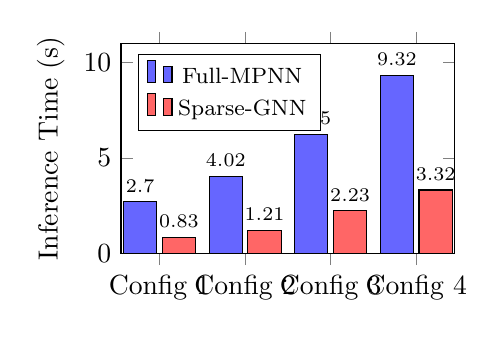
\begin{tikzpicture}
\begin{axis}[
    ybar,
    bar width=12pt,
    enlarge x limits=0.15,
    legend style={at={(0.05,0.95)}, anchor=north west, font=\footnotesize},
    ylabel={Inference Time (s)},
    symbolic x coords={Config 1, Config 2, Config 3, Config 4},
    xtick=data,
    nodes near coords,
    every node near coord/.append style={font=\scriptsize},
    width=0.48\textwidth,
    height=0.35\textwidth,
    ymin=0, ymax=11
]
\addplot[fill=blue!60] coordinates {(Config 1, 2.70) (Config 2, 4.02) (Config 3, 6.25) (Config 4, 9.32)};
\addlegendentry{Full-MPNN}
\addplot[fill=red!60] coordinates {(Config 1, 0.83) (Config 2, 1.21) (Config 3, 2.23) (Config 4, 3.32)};
\addlegendentry{Sparse-GNN}
\end{axis}
\end{tikzpicture}